%------------------------------------------
%       $Id: GMT_API.tex,v 1.2 2006-04-01 04:20:19 pwessel Exp $
%
%       The GMT Documentation Project
%       Copyright 2000-2006.
%       Paul Wessel and Walter H. F. Smith
%------------------------------------------
%
\documentclass{report}

\usepackage{ifpdf}
%\usepackage{epsfig}
\usepackage{graphicx}
\usepackage{makeidx}
\usepackage{a4wide}
\usepackage{float}
\usepackage{html}
\usepackage{GMT}
\usepackage{times}
\usepackage{color}
\usepackage{mathptm}

\ifpdf
%  \usepackage[pdftex, linkbordercolor={1 1 0}, bookmarksnumbered=true,
%  boolmarksopenlevel=3, urlbordercolor={1 0 0}]{hyperref}
  \usepackage[pdftex]{hyperref}
  \pdfcompresslevel=9
  \DeclareGraphicsExtensions{.pdf}

 \hypersetup{%
    pdftitle={The Generic Mapping Tools Version 5---The GMT API},
    pdfauthor={Paul Wessel,  Walter H. F. Smith},
    pdfkeywords={GMT, projections, mapping},
    book,arksopen=true,
    bookmarksnumbered,
    %pdfstartview={FitH},
    %linkbordercolor={1 1 0},
    %urlbordercolor={1 0 0},
  }%

\else
   \DeclareGraphicsExtensions{.eps}
\fi



% Special commands & environments for GMT documentation
%
%       GMTfig will insert an eps file, add a label, and set a caption
%

\newcommand{\GMTfig}[3][tbp]{\begin{figure}[#1] \centering \includegraphics{eps/#2} \caption{#3} \label{fig:#2}  \end{figure}}

\newcommand{\PS}{\textit{PostScript}}
\newcommand{\UNIX}{\textit{UNIX}}


\ifpdf
\newcommand{\GMTprog}[1]{\htmladdnormallink{{\textsf{\textbf{#1}}}}{../html/#1.html}\index{#1@{\textsf{\textbf{#1}}}}}
\newcommand{\GMTprogi}[1]{\htmladdnormallink{{\textsf{\textbf{#1}}}}{../html/#1.html}}
\else
\newcommand{\GMTprog}[1]{\htmladdnormallink{{\textsf{\textbf{#1}}}}{../#1.html}\index{#1@{\textsf{\textbf{#1}}}}}
\newcommand{\GMTprogi}[1]{\htmladdnormallink{{\textsf{\textbf{#1}}}}{../#1.html}}
\fi

\newcommand{\filename}[1]{\underline{#1}}
\newcommand{\gmt}{\htmladdnormallink{\textbf{GMT}}{http://gmt.soest.hawaii.edu}}
%%------------ THESE COMMANDS WILL BE EXCLUDED WHEN HTML VERSION IS MADE--------

\ifpdf%DVIGMT
\newcommand{\GMT}{\textit{GMT}}%DVIGMT
\else%DVIGMT
\newcommand{\GMT}{\htmladdnormallink{\includegraphics{eps/GMT_glyph10.eps}}{http://gmt.soest.hawaii.edu}}%DVIGMT
\fi%DVIGMT

\newcommand{\DS}{$^{\circ}$}%DVIGMT
\newcommand{\progname}[1]{{\textsl{\textbf{#1}}}\index{#1@{\textsl{\textbf{#1}}}}}%DVIGMT
\newcommand{\Opt}[1]{{\bf --#1}}%DVIGMT
\newcommand{\startscript}{\scriptsize}%DVIGMT
\newcommand{\stopscript}{\normalsize}%DVIGMT
%%------------------------------------------------------------------------------

%%------------ THESE COMMANDS WILL BE EXCLUDED WHEN DVI VERSION IS MADE---------
\newcommand{\GMT}{\htmladdnormallink{\textbf{GMT}}{http://gmt.soest.hawaii.edu}}%HTMLGMT
\newcommand{\progname}[1]{{\textit{#1}}\index{#1@{\textit{#1}}}}%HTMLGMT
\newcommand{\Opt}[1]{{\bf -#1}}%HTMLGMT
\newcommand{\DS}{$^{o}$}%HTMLGMT
\newcommand{\startscript}{}%HTMLGMT
\newcommand{\stopscript}{}%HTMLGMT
\include{GMT_version}


%--------------------------------------------------------------------------

\pagecolor{white}

\makeindex

\begin{document}
\pagenumbering{roman}

\pagestyle{headings}

\thispagestyle{empty}

\begin{center}
\huge
\textbf{The Generic Mapping Tools}\par 
\vspace{0.5\baselineskip}


\includegraphics{eps/GMT_covertext} 

\huge
\textbf{\GMTDOCVERSION}\par 
\vspace{0.25\baselineskip}

\Huge
\textbf{Application Programming Interface}\par 

\large
\vspace{0.75\baselineskip}
\textbf{by}\par 
\vspace{0.75\baselineskip}

\huge
\textbf{P\aa l (Paul) Wessel}\par 
\vspace{0.5\baselineskip}

\Large
\textbf{School of Ocean and Earth Science and Technology}\par 
\textbf{University of Hawai'i at M\={a}noa}\par 

\large
\vspace{0.75\baselineskip}
\textbf{and}\par 
\vspace{0.75\baselineskip}

\huge
\textbf{Walter H. F. Smith}\par 
\vspace{0.5\baselineskip}

\Large
\textbf{Laboratory for Satellite Altimetry}\par 
\textbf{NOAA/NESDIS/NODC}\par 
\vspace{0.5\baselineskip}

\large
\textbf{\GMTDOCDATE}\par 
\vspace{\baselineskip}

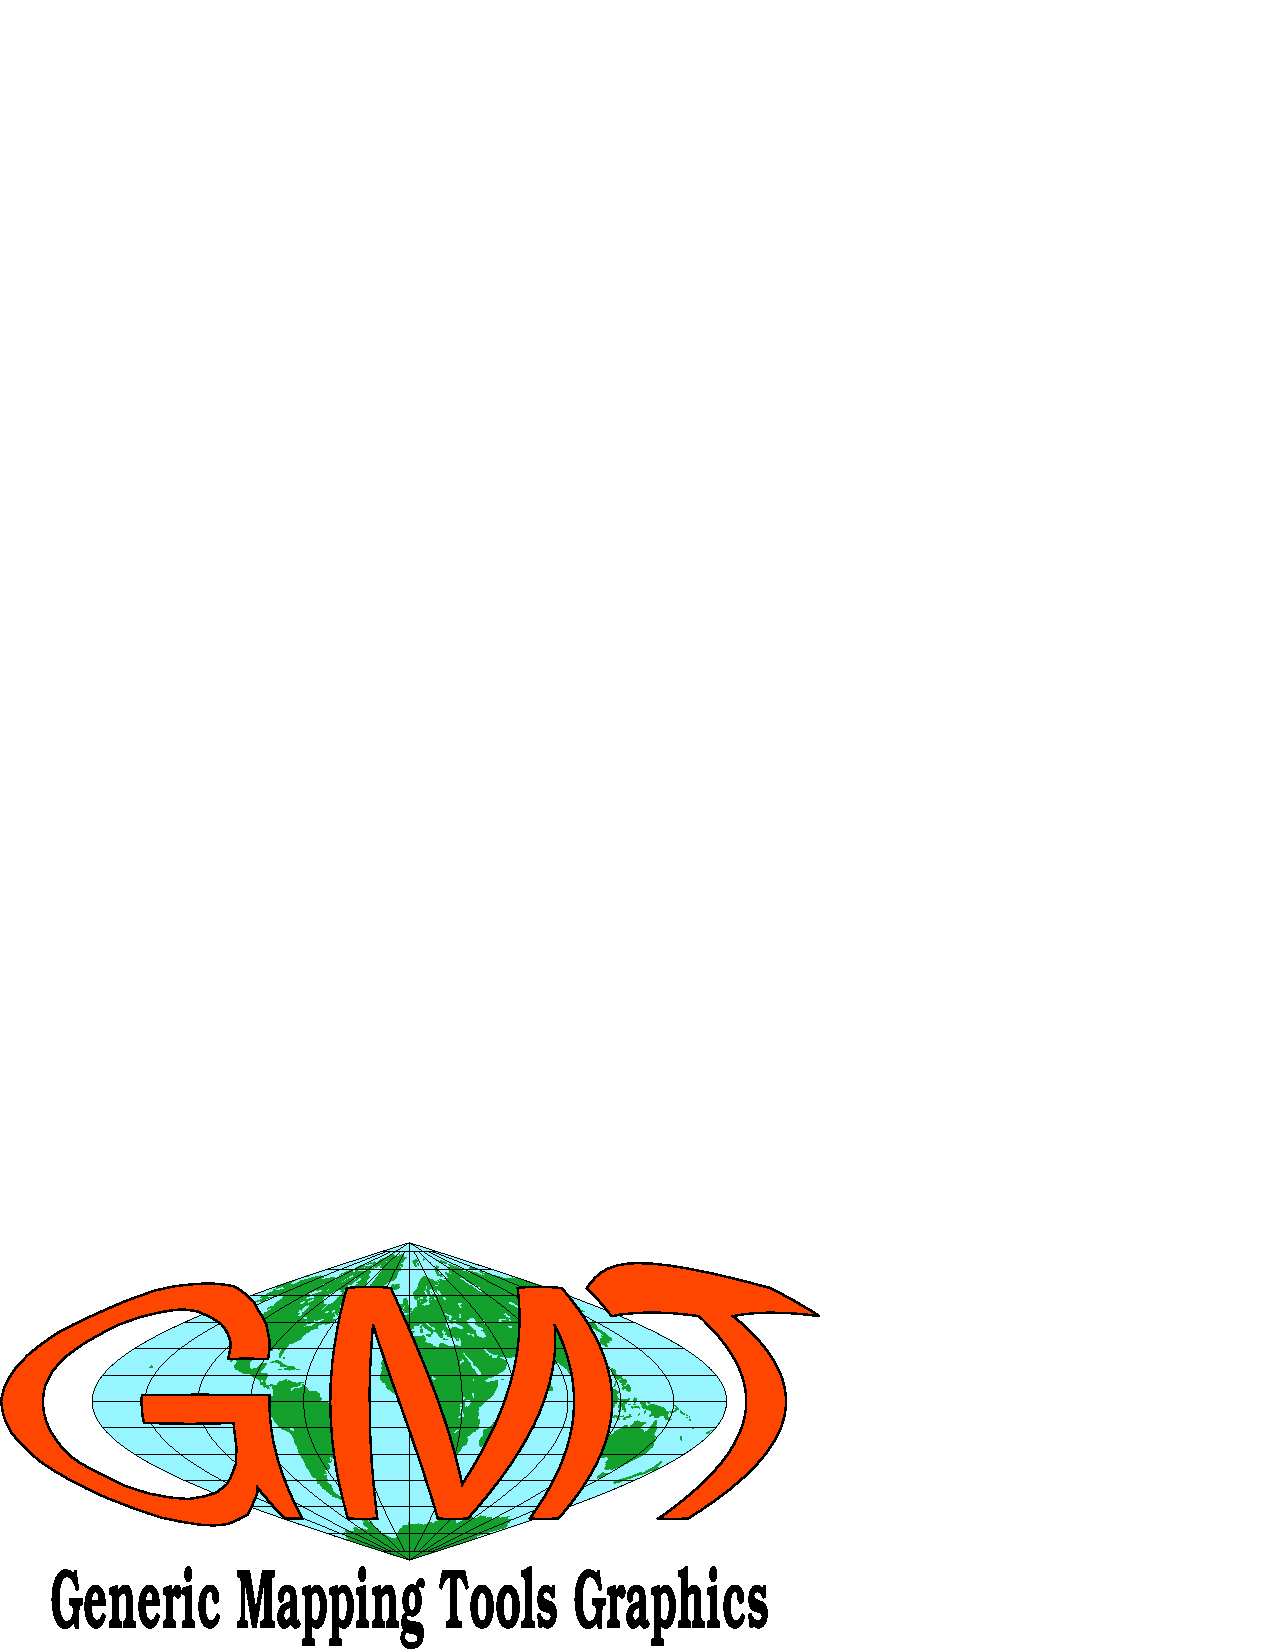
\includegraphics{eps/GMT_coverlogo}

\end{center}
\clearpage

\thispagestyle{headings}

\tableofcontents 
\thispagestyle{headings}

\chapter*{INTRODUCTION} 
\pagenumbering{arabic}
\thispagestyle{headings}
\addcontentsline{toc}{chapter}{INTRODUCTION}
\index{Purpose of API}

This documentation serves two related purposes:
\begin{enumerate}
\item It will document the \GMT\ API library for application developers that wish
to call functions in the API.
\item It will document the underlying \GMT\ API utilities for developers of
the API itself.
\end{enumerate}
Of course, many developers might be interested in learning about both sets of
functions.\\

\section*{\gmt\ Overview of the GMT Application Program Interface}
\addcontentsline{toc}{section}{\gmt\ Overview of the GMT Application Program Interface}

Users who wish to create their own GMT-like applications based on the API
must make sure their program goes through these steps:

\subsection*{Historical highlights}
\addcontentsline{toc}{subsection}{Historical highlights}
\index{GMT@\GMT!history}

\begin{enumerate}
\item Initialize a GMT session by calling \texttt{GMTAPI\_Create\_Session} which
will return a pointer to a GMT API control structure.  This pointer will be used
as the first argument to all subsequent GMT API function calls.
\item Register any input sources and output destinations with the session using
\texttt{GMTAPI\_Register\_Import} and \texttt{GMTAPI\_Register\_Export}, respectively.
These will typically be used to specify memory locations and open file handles;
i/o involving files are already handled by GMT itself.
\item Each registration will generate a unique ID number.  These numbers are to be
used with the relevant GMT function as filenames of the form ``GMTAPI-\#-ID''.  When
GMT  functions encounter such filenames they will extract the ID and make a connection
to the source of destination registered under that ID.
\item When a source or destination is no longer needed, you should free it up by calls
to ?.
\item Repeat steps 2--4 as many times as your application desires.  All functions
return a status code which is 0 if all is well.  For non-zero return values, use
\texttt{GMTAPI\_Report\_Error} to generate an error message on {\it stderr}.
\item To terminate the GMT session, call \texttt{GMTAPI\_Destroy\_Session}.
\end{enumerate}

\subsection*{The GMT Application Program Interface}
\addcontentsline{toc}{subsection}{The GMT Application Program Interface}
\index{GMT@\GMT!Interface}

All calls to the GMT functions themselves have identical syntax that come in two different flavors.
They differ in how the command options are passed to the function which can be done via
\begin{enumerate}
\item a text-based command specification.
\item A pointer to a GMT common option structure and a linked list of objects with individual options
for the current program.
\end{enumerate}

The former interface is used by the stand-alone GMT applications and is expected to be used by
FORTRAN developers; however, there are no restrictions on the use of these functions.  The
latter interface allows developers of higher-level programming languages to pass all command
options via a common structure with the basic GMT domain and projection options as well as a
NULL-terminated, linked list of structures, each containing information about one program option.
The syntax of the two formats are:

\texttt{int GMT\_program\_cmd (struct GMTAPI\_CTRL *API, int n\_args, char *args[])}
\texttt{int GMT\_program (struct GMTAPI\_CTRL *API, struct GMT\_COMMON *C, struct GMT\_OPTIONS *options)}

where ``program'' is replaced by the desired application name (e.g., blockmean, psxy, grdmath).


\chapter{SESSION ONE} 
\thispagestyle{headings}

\section{Tutorial setup}
\begin{enumerate}

\item We assume that \GMT\ has been properly and fully
installed and that you have the statement
\texttt{setenv GMTHOME $<$path to \GMT\ directory$>$}
in your \filename{.login} as
described in the \GMT\ \filename{README} file.

\item All \GMT\ man pages, documentation, and example scripts
are available from the \GMT\ documentation web page.  It is
assumed these pages have been installed locally at your site;
if not they are always available from the main
\htmladdnormallinkfoot{GMT home page}{http://gmt.soest.hawaii.edu}.
\end{enumerate}

\chapter{References} 
\thispagestyle{headings}

\begin{enumerate}

\item Smith, W.H.F., and P. Wessel, Gridding with continous curvature
splines in tension, {\it Geophysics}, {\it 55}, 293--305, 1990.

\item Wessel, P., and W.H.F. Smith, Free software helps map and
display data, {\it EOS Trans. AGU}, {\it 72}, 441, 1991.

\item Wessel, P., and W.H.F. Smith, New version of the Generic
Mapping Tools released, {\it EOS Trans. AGU}, {\it 76}, 329, 1995.

\item Wessel, P., and W.H.F. Smith, A global, self-consistent,
hierarchical, high-resolution shoreline database, {\it J. Geophys. Res.},
{\it 101}, 8741--8743, 1996.

\item Wessel, P., and W.H.F. Smith, New, improved version of the Generic
Mapping Tools released, {\it EOS Trans. AGU}, {\it 79}, 579, 1998.

\item Wessel, P., and W.H.F. Smith, The Generic Mapping Tools Technical Reference and Cookbook, {\it Version 4.0}, pp. 132, 2004.

\end{enumerate}

\clearpage
\thispagestyle{headings}
\addcontentsline{toc}{chapter}{INDEX}
\printindex
\thispagestyle{headings}

\end{document}
